\section{Dataset}\label{section:dataset}

The first part of ISBI Challenge 2017 \cite{codella2018skin} - Skin Lesion Analysis Towards Melanoma Detection: Lesion Segmentation dataset is used in this thesis.
This dataset has train, validation and test data separately. The training dataset consist of 2000 dermoscopic .jpg images and the related masks with .png format.
The dataset include various type of lesions namely malignant melanoma, nevus and seborrhoeic keratosis.
Sample images is given with corresponding masks in Figure ~\ref{figure:sample-images-from-dataset}.

\begin{figure}
    \centerline{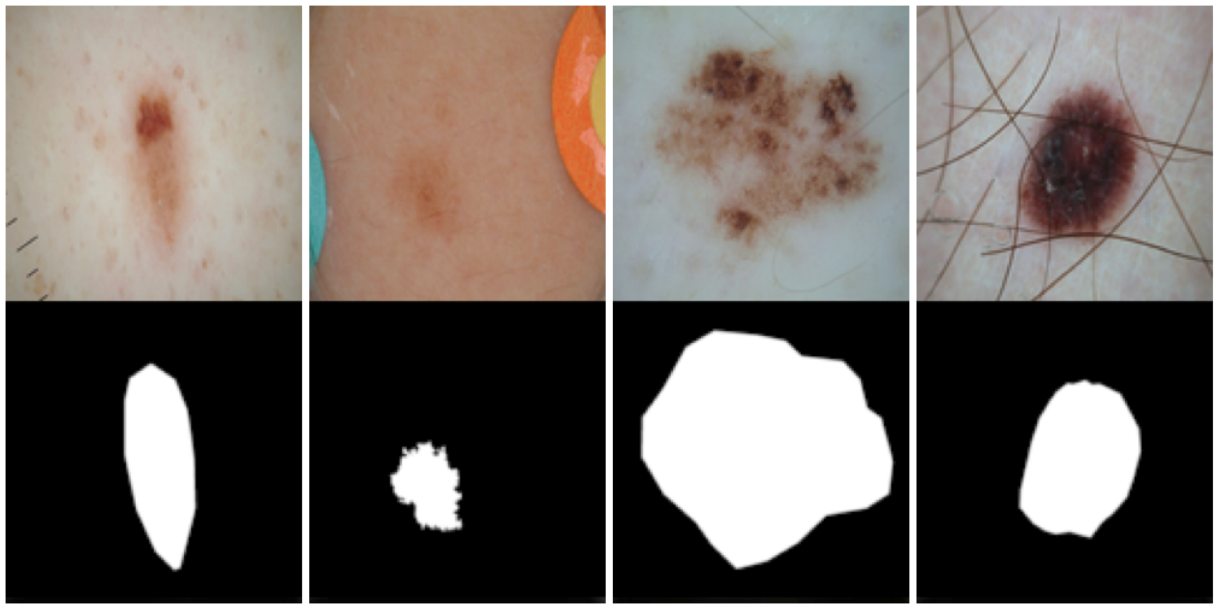
\includegraphics[width=1\columnwidth]{04-methodology/figures/sample-images-from-dataset.png}}
    \caption{Sample images from dataset. First row is original images, second row is corresponding masks}
    \label{figure:sample-images-from-dataset}
\end{figure}

There are also validation and test datasets which contain 150 and 600 images respectively.
The results are based on several common image similarity metrics which are given related section.

\begin{figure}
    \centerline{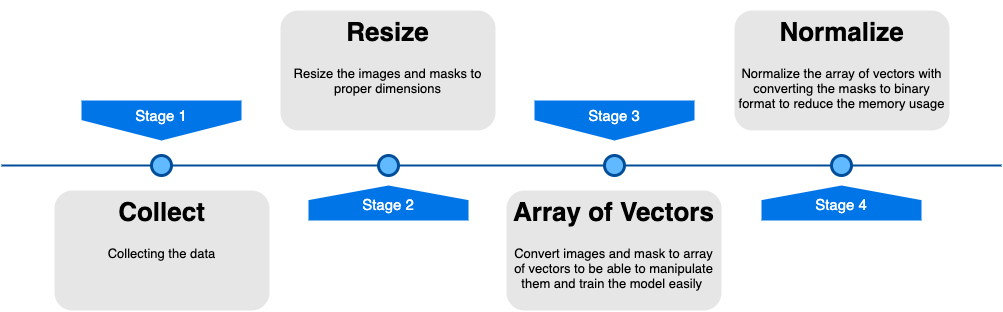
\includegraphics[width=1\columnwidth]{04-methodology/figures/data-preparation-process.png}}
    \caption{Data preparation process}
    \label{figure:data-preparation-process}
\end{figure}

The images are of various dimensions and the all used neural networks can't handle relatively big images because of their different internal architectures and memory constraints.
We also had to resize all images into same dimension to reduce the memory consumption and increase the accuracy as a preprocessing stage.
As it can be stated at Figure~\ref{figure:data-preparation-process}, arrays of mask files converted to uint8 to reduce the size of the masks.
